\documentclass{standalone}
\usepackage{tikz}
\usetikzlibrary{positioning}
\begin{document}
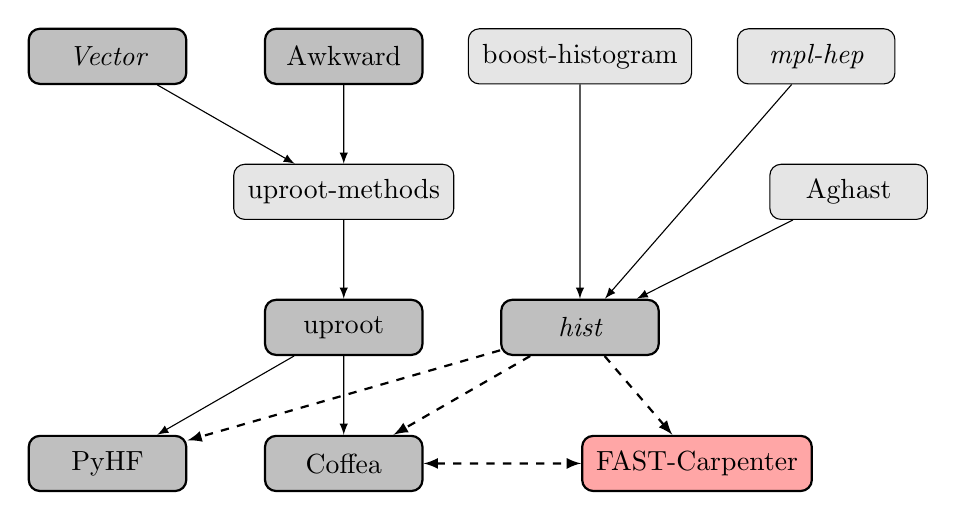
\begin{tikzpicture}[scale=3,
every node/.style={},
package/.style={node distance=3cm, rectangle, draw, fill=black!10, inner sep=5pt, rounded corners, minimum width=2cm, minimum height=.7cm},
user/.style={fill=black!25, thick},
planned/.style={font=\itshape},
external/.style={fill=red!35},
existing/.style={-latex},
desired/.style={dashed, thick, -latex}
]

\node [package, user, planned] (vector) {Vector};
\node [package, user] (awkward) [right of=vector] {Awkward};
\node [package] (bh) [right of=awkward] {boost-histogram};
\node [package, planned] (mplhep) [right of=bh] {mpl-hep};

\node [package]  (uprootmeth) [below=1cm of awkward] {uproot-methods};
\node [package] (aghast) [right=4cm of uprootmeth] {Aghast};

\node [package, user] (uproot) [below=1cm of uprootmeth] {uproot};
\node [package, user, planned]  (hist) [right of=uproot] {hist};

\node [package, user] (coffea) [below=1cm of uproot] {Coffea};
\node [package, user] (pyhf) [left of=coffea] {PyHF};
\node [package, user, external] (fast) [right=2 cm of coffea] {FAST-Carpenter};

\draw [existing] (bh) -- (hist);
\draw [existing] (mplhep) -- (hist);

\draw [existing] (vector) -- (uprootmeth);
\draw [existing] (awkward) -- (uprootmeth);
\draw [existing] (uprootmeth) -- (uproot);
\draw [existing] (aghast) -- (hist);

\draw [existing] (uproot) -- (coffea);
\draw [desired] (hist) -- (coffea);

\draw[desired, latex-latex] (coffea) -- (fast);
\draw[desired] (hist) -- (fast);

\draw[existing] (uproot) -- (pyhf);
\draw[desired] (hist) -- (pyhf);

\end{tikzpicture}
\end{document}
